% Report 2: revised research report. Build with: python scripts/build_report2.py
% Every quantitative result is a \val{...} macro or a generated table produced from
% results/report2/analysis by scripts/build_report2.py; no result is typed by hand.
\documentclass[runningheads]{llncs}
\usepackage[T1]{fontenc}
\input{generated/fonts.tex}% Times via newtx when it loads cleanly, otherwise the default font
\usepackage{graphicx}
\usepackage{booktabs}
\usepackage{tabularx}
\usepackage{float}
\usepackage{amsmath}
\usepackage{tikz}
\usetikzlibrary{positioning,arrows.meta,calc}
\usepackage[hidelinks]{hyperref}
\usepackage{xcolor}
\renewcommand\UrlFont{\color{blue!60!black}\rmfamily}
\urlstyle{rm}
\graphicspath{{figures/}}
\setlength{\emergencystretch}{1.5em}
\raggedbottom
\input{generated/values.tex}
\newcommand{\dd}{\textsuperscript{\dag}}
\newcolumntype{R}{>{\raggedleft\arraybackslash}X}
\hypersetup{pdftitle={Evaluating the Economic Value and Operational Reliability of LLM-Assisted Retail Decisions under Demand and Supply Shocks},
            pdfauthor={Nguyen Thai Duy}}

\begin{document}

\title{Evaluating the Economic Value and Operational Reliability of LLM-Assisted Retail Decisions under Demand and Supply Shocks}
\subtitle{Second research report, revised after review}
\titlerunning{LLM-Assisted Retail Decisions under Shocks}
\author{\texorpdfstring{Nguy\~{\^e}n Th\'ai Duy}{Nguyen Thai Duy}}
\authorrunning{Nguy\~{\^e}n Th\'ai Duy}
\institute{Research report, 3 November 2026\\
\url{https://github.com/DnyChillTypin/llm-business-shocks-sim}}
\maketitle

\begin{abstract}
We test whether a large language model (LLM) adds economic value when it sets daily prices and replenishment orders for a simulated retailer facing demand and supply shocks. The study responds to a review of our first report by redesigning the experiment around a frozen protocol: 36 distinct store--product--window blocks drawn from a synthetic retail dataset (\val{int.prefix_groups} block--elasticity groups across cohorts), four conditions (no shock, demand surge, demand decline, delivery disruption) branched from an identical pre-shock state, three repeated LLM runs per condition, explicit history ablations, and fresh LLM runs at three price elasticities. In total we analyse \val{int.llm_branches} LLM trajectories (\val{rel.total.completed_decisions} decisions) and \val{int.baseline_branches} rule-based trajectories. The evaluated system is a composite policy: \texttt{gpt-4.1-mini} with one repair attempt and an adaptive fallback rule. It earns less contribution than a simple adaptive replenishment rule in all but \val{main.cells_llm_ahead} of \val{main.cells_total} block--condition comparisons, with mean contrasts between \val{main.raw_vs_adaptive.demand_decline.mean} and \val{main.raw_vs_adaptive.demand_surge.mean} simulator units per 14-day response period. In accounting terms the gap is exactly lower gross margin plus higher holding cost. The policy discounts often and accumulates stock, behaviour consistent with both components, although the prompt states the cost structure and elasticity; we present this as an interpretation, not a tested causal attribution. Rolling sales history does not help: frozen and no-history variants earn more on average in every condition. The negative result holds at elasticities 0.75 and 2.25. The first model response is valid for \val{rel.main.first_pass_valid_share} of decisions, and \val{rel.main.fallback_share} fall back to the rule. Within this simulator, the evidence supports a negative conclusion about the policy's economic value.

\keywords{Large language models \and Retail operations \and Inventory and pricing \and Demand shocks \and Supply disruption \and Simulation \and Negative results}
\end{abstract}

% =====================================================================
\section{Introduction}

Language models are increasingly proposed as decision aids for operational choices such as pricing and replenishment. Whether they add economic value is an empirical question. Answering it requires an outcome measure that reflects business consequences rather than answer quality, a credible comparator, and a design that separates the policy's response from incidental differences in its starting position.

Our first report~\cite{report1} compared an LLM retail policy with fixed and adaptive replenishment rules under demand and delivery shocks. The LLM policy exceeded the adaptive rule in \val{legacy.raw_pos} of 9 shock comparisons. Its review identified four issues that prevented any conclusion about adaptation:
\begin{itemize}
\item the study used only three selected store--product series and one LLM run per condition;
\item the LLM's actions already differed between shock and control runs before the shock began (\val{legacy.diverged} of 9 pairs);
\item outcomes conflated the model with its repair and fallback machinery;
\item the price-sensitivity analysis covered only the rule-based baselines.
\end{itemize}

This report answers those points with a redesigned experiment whose protocol, sample and estimands were frozen on 31 October 2026, before any evaluation outcome was generated. We ask four questions:
\begin{description}
\item[RQ1] Does the composite LLM policy improve contribution relative to an adaptive rule under shocks?
\item[RQ2] Does explicit, updated sales history improve the policy's response?
\item[RQ3] How much repair, fallback, latency and API expense does the policy require?
\item[RQ4] Do the conclusions persist when the assumed price elasticity changes?
\end{description}

The contributions are threefold. First, a matched-prefix branching protocol that restores an identical simulator state before the shock for every policy, history variant and condition, so post-shock differences cannot come from earlier divergence. Second, a completed evaluation of \val{int.llm_branches} LLM and \val{int.baseline_branches} rule-based trajectories with full accounting of every model request, repair, fallback, interruption and cost. Third, an exact accounting decomposition of the shortfall into gross margin and holding cost, together with descriptive evidence of two behaviours consistent with it, discounting and overstocking, which the policy exhibits even though its instructions contain the information needed to avoid them. The answer to RQ1 is negative, and we report it as such.

% =====================================================================
\section{Positioning}\label{sec:positioning}

RetailBench~\cite{retailbench2026} evaluates LLM agents on long-horizon autonomous retail management. We reuse its inventory, order and supplier components at a pinned commit~\cite{retailbench_code}, but the evaluation differs in purpose and form:
\begin{itemize}
\item episodes are 21 days long and driven by store--product demand series from a public synthetic dataset~\cite{kaggle_retail_v8};
\item the model returns one JSON object per day containing an order quantity and a price multiplier, rather than operating as a tool-using agent;
\item shocks are scheduled interventions on otherwise identical branches;
\item outcomes are paired against rule-based comparators from the same starting state.
\end{itemize}
Our scores are therefore not comparable with RetailBench scores. The contribution here is a controlled shock-response protocol with economic outcomes and operational reliability accounting, not a new benchmark.

Following the review, this report is restricted to the retail study. The first report's separate native benchmark track (reasoning, consulting and strategy tasks) addressed different questions and is not continued here. Results from the first report are kept separate from the new evidence (Appendix~\ref{app:legacy}), and the two cohorts' denominators are never pooled.

% =====================================================================
\section{Study design}\label{sec:design}

\subsection{Data and sampling}

The demand source is version~8 of a public synthetic retail dataset~\cite{kaggle_retail_v8}. It contains 76{,}000 daily rows for 100 store--product series from 1~January 2022 to 30~January 2024, and its CSV hash is recorded in the protocol. The data are synthetic and the source had been inspected during earlier work, so we make no claim of evaluation on unseen real data.

Series were selected by a deterministic rule that uses only the training period, which ends 1~April 2023. Eligible series exclude the three used in the first report and are ranked by the coefficient of variation of training demand. Twelve are taken at evenly spaced quantiles. Each series is evaluated in three non-overlapping 21-day windows between 3~November 2023 and 4~January 2024, giving 36 \emph{blocks}. A preselected subset of six series (\val{int.diagnostic_blocks} blocks) is used for the history and elasticity cohorts. Two development cases from mid-2023 were used only for engineering and costing, and are excluded from all results.

\subsection{Simulator}

Each day the simulator converts a series' base demand $D_t$ into requested demand
\begin{equation}
q_t = \left\lfloor D_t \, s_t \, m_t^{-\varepsilon} + \tfrac12 \right\rfloor,
\end{equation}
where $m_t \in \{0.9, 1.0, 1.1\}$ is the chosen price multiplier, $\varepsilon$ is the price elasticity (reference value 1.5) and $s_t$ is the shock multiplier. The shock multiplier is 1.5 for a demand surge and 0.7 for a demand decline on days 8--14, and 1 otherwise. A delivery disruption raises the supplier lead time from 2 to 5 days on days 8--14.

Unit cost is \val{econ.cost_ratio} of the reference price, and daily holding cost is $0.001$ times unit cost per unit of closing stock. Unmet demand is lost. The primary outcome is \emph{contribution} over the response period, days 8--21:
\begin{equation}
C = \sum_{t=8}^{21} \bigl[\, \text{sales}_t\,(p_t - c) - h_t \,\bigr],
\end{equation}
where $p_t$ is the price, $c$ the unit cost and $h_t$ the holding cost. Contribution is not full business profit: there are no fixed costs, and stock carried past day 21 retains its purchase-cost value outside $C$. All monetary values are in the dataset's synthetic units and are unrelated to API expenditure.

\subsection{Matched-prefix branching}

Days 1--7 of every block are run once with the adaptive rule. The complete state is then saved immediately before day 8: cash, stock lots, outstanding orders, prices, date, history, accounting state and random-number state. Every branch of that block restores this snapshot (Fig.~\ref{fig:design}). Because each elasticity setting has its own warm-up, the 36 blocks give \val{int.prefix_groups} block--elasticity groups: 36 at the reference elasticity and 18 at each of the other two. Within a block and elasticity setting, corresponding branches differ only in the scheduled condition, the policy, and the history treatment. Days 8--21 are the evaluated period; days 1--7 are common by construction.

The estimand is therefore the performance of a policy that takes over a business from a common state. It is not the outcome of deploying the policy from day~1. For every one of the \val{int.prefix_groups} block--elasticity groups, all \val{int.llm_branches} LLM and \val{int.baseline_branches} baseline branches restored an identical prefix and an identical restored-state hash.

\begin{figure}[t]
\centering
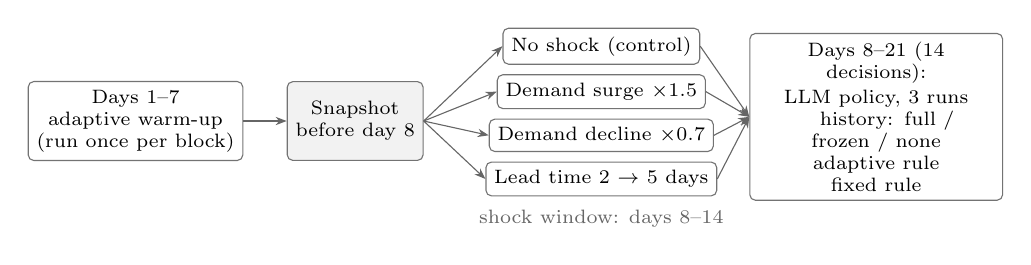
\begin{tikzpicture}[
  box/.style={draw=black!55, rounded corners=2pt, align=center, font=\scriptsize, inner sep=3pt},
  arr/.style={-{Stealth[length=4pt]}, black!60}]
\node[box, minimum width=2.4cm, minimum height=1.0cm] (warm) {Days 1--7\\adaptive warm-up\\(run once per block)};
\node[box, right=0.55cm of warm, minimum height=1.0cm, fill=black!5] (snap) {Snapshot\\before day 8};
\node[box, right=1.0cm of snap, yshift=0.95cm, minimum width=2.1cm] (c1) {No shock (control)};
\node[box, below=0.12cm of c1, minimum width=2.1cm] (c2) {Demand surge $\times1.5$};
\node[box, below=0.12cm of c2, minimum width=2.1cm] (c3) {Demand decline $\times0.7$};
\node[box, below=0.12cm of c3, minimum width=2.1cm] (c4) {Lead time 2 $\to$ 5 days};
\node[box, right=0.55cm of c2, yshift=-0.32cm, minimum width=3.1cm, minimum height=1.6cm, text width=3.0cm] (pol)
  {Days 8--21 (14 decisions):\\[1pt] LLM policy, 3 runs\\ \quad history: full / frozen / none\\ adaptive rule \\ fixed rule};
\draw[arr] (warm) -- (snap);
\foreach \c in {c1,c2,c3,c4} { \draw[arr] (snap.east) -- (\c.west); \draw[arr] (\c.east) -- (pol.west); }
\node[font=\scriptsize, black!60, below=0.05cm of c4] {shock window: days 8--14};
\end{tikzpicture}
\Description{Diagram: a seven-day adaptive warm-up produces a saved snapshot, which is restored into four condition branches; each branch is run by the LLM policy and the two rule baselines for days 8 to 21.}
\caption{Matched-prefix design. Each block's state before day~8 is restored into every condition, policy and history variant. The same design is repeated separately at each elasticity.}\label{fig:design}
\end{figure}

\subsection{Policies}

The \textbf{LLM policy} is a composite system built on the model \texttt{gpt-4.1-mini} (snapshot dated 14 April 2025), which receives one request per day through a commercial API gateway (temperature 0, at most 1{,}024 output tokens, 90-second timeout, no automatic retries). The fixed system prompt states the objective (cumulative contribution), the cost structure, the holding-cost rate, the assumed elasticity, the allowed price multipliers, lead times, and the JSON action schema. The daily observation gives cash, stock, outstanding orders, unit cost, reference demand, and up to 14 completed days of price-normalised demand history.

An invalid response triggers one repair request that quotes the validation errors. If the repair is also invalid, the adaptive rule chooses that day's action from the same observation (\emph{fallback}). A transport or budget failure stops the branch rather than invent an action. Such branches were re-run from the snapshot after review, with their costs retained. There is no conversational memory across days. The gateway's served model identity is not independently attested.

The \textbf{adaptive rule} estimates mean demand from the last 14 days of history and orders up to five days of that demand, net of stock on hand and on order. It prices at 1.1 when stock covers fewer than two days of demand, at 0.9 when it covers more than seven, and at 1.0 otherwise. The \textbf{fixed rule} orders up to five days of the training-period mean demand and always prices at 1.0. Both are deterministic and run once per block and condition.

\textbf{History variants} change only the history field of the LLM's observation after day~7. \emph{Full} history is the rolling last 14 completed days. \emph{Frozen} history is the history available at the end of day~7, left unchanged. \emph{No history} is an explicitly empty field. The same treatment is applied to the fallback rule's input, so the ablation measures the composite policy's dependence on history. Current stock and cash still carry the consequences of the past.

\subsection{Cohorts}

Table~\ref{tab:cohorts} lists the frozen experiment matrix. The full-history main-cohort runs on the diagnostic blocks serve as the reference for the history cohort, and as the elasticity-1.5 setting for the elasticity cohort. No duplicate runs were purchased.

\begin{table}[t]
\caption{Experiment matrix. Each LLM branch has 14 decisions.}\label{tab:cohorts}
\centering\footnotesize
\begin{tabularx}{\textwidth}{@{}l X r r@{}}
\toprule
Cohort & Design & LLM branches & Decisions \\
\midrule
Main & 36 blocks $\times$ 4 conditions $\times$ 3 runs; full history; $\varepsilon=1.5$ & 432 & 6{,}048 \\
History & 18 blocks $\times$ 4 conditions $\times$ 3 runs $\times$ \{frozen, none\} & 432 & 6{,}048 \\
Elasticity & 18 blocks $\times$ 4 conditions $\times$ 3 runs $\times$ $\varepsilon \in \{0.75, 2.25\}$ & 432 & 6{,}048 \\
Baselines & adaptive and fixed: 36 blocks $\times$ 4 at 1.5; 18 blocks $\times$ 4 at 0.75 and 2.25 & 576 rule & 8{,}064 \\
\bottomrule
\end{tabularx}
\end{table}

\subsection{Estimands and analysis}

For condition $k$ in block $b$, let $\bar C^{\text{LLM}}_{bk}$ be the mean contribution over the three LLM runs and $C^{\text{A}}_{bk}$ the adaptive rule's contribution. The \emph{raw contrast} is $\Delta_{bk} = \bar C^{\text{LLM}}_{bk} - C^{\text{A}}_{bk}$. The \emph{control-adjusted interaction} for a shock $k$ is
\begin{equation}
I_{bk} = \bigl(\bar C^{\text{LLM}}_{bk} - \bar C^{\text{LLM}}_{b0}\bigr) - \bigl(C^{\text{A}}_{bk} - C^{\text{A}}_{b0}\bigr) = \Delta_{bk} - \Delta_{b0},
\end{equation}
where $k=0$ is the no-shock control. A positive $I_{bk}$ means the LLM policy lost less to the shock than the adaptive rule did. It does not mean the LLM policy earned more. History contrasts are full minus frozen and full minus none, computed the same way. Blocks are weighted equally.

The analysis is descriptive. Blocks share stores, products and calendar periods, and the three LLM runs measure the variability of model responses rather than independent businesses. Following the frozen protocol, we report means, medians, ranges and sign counts, and no confidence intervals or significance tests.

A shocked trajectory is \emph{recovered} at the first day $d \in \{15,\dots,19\}$ that begins three consecutive days with zero lost sales and closing stock within 20\% of its own paired control trajectory's stock (relative to the larger of that stock and 1). The recovery delay is $d-14$, and trajectories that do not recover by day~21 are right-censored.

% =====================================================================
\section{Execution, integrity and deviations}\label{sec:execution}

All planned branches were completed and validated: \val{int.llm_branches} LLM and \val{int.baseline_branches} baseline trajectories, with \val{int.daily_rows} daily records. For every branch, three checks pass:
\begin{itemize}
\item daily contribution reconciles with the branch summary;
\item replaying the recorded actions reproduces the trajectory exactly;
\item every executed decision is exactly one of a valid first response, a successful repair, or a fallback.
\end{itemize}

Table~\ref{tab:ops} shows the cost of execution. A branch whose run stopped was archived and restarted from its snapshot under supervision. There were \val{rst.total.restart_events} such restart events across \val{rst.total.distinct_branches} distinct branches, since some branches stopped more than once. The stopping request failed with a timeout in \val{rst.total.cause_timeout} events, a process interruption with unknown gateway outcome in \val{rst.total.cause_process_interrupted}, a connection error in \val{rst.total.cause_connection_error}, a gateway server error (HTTP \val{rst.total.server_error_http}) in \val{rst.total.cause_server_error}, and a rate-limit response in \val{rst.total.cause_rate_limit}; the remaining \val{rst.total.cause_no_failed_request} restarts had no failed request. The interrupted runs added \val{ops.total.attempts_in_interrupted_runs} requests whose results are excluded from outcomes but whose costs are retained. When a failed request's charge is unknown, its full reservation is held as an \emph{unknown-charge reserve}. This applied to \val{rst.total.restarts_with_reserve} restarts, \val{ops.total.unknown_charge_reserves} credits in total; the \val{rst.total.cause_no_failed_request} restarts without a failed request held none. One main-cohort restart receipt records an approved hold slightly different from its proposal; the ledger retains the full proposal reserve, which is the value reported here. Total project exposure, including earlier work and all reserves, is \val{ops.project_exposure} of a 20-credit budget.

\begin{table}[t]
\caption{Execution cost by cohort, including interrupted runs. Restart events count supervised restarts; a branch can restart more than once, so the next column counts distinct branches restarted. Credits are gateway credits estimated from observed tokens at published rates; unknown charges are held at their full reserve.}\label{tab:ops}
\centering\footnotesize
\begin{tabular*}{\textwidth}{@{\extracolsep{\fill}}l r r r r r r r@{}}
\toprule
& & In interrupted & Restart & Branches & Known & & \\
Cohort & Requests & runs & events & restarted & credits & Reserves & Exposure \\
\midrule
\input{generated/tab_operations.tex}
\end{tabular*}
\end{table}

\paragraph{Protocol deviation.} During the elasticity cohort, the request timeout was raised from the frozen 90~seconds to 180~seconds after repeated gateway timeouts. Main and history cohorts are unaffected. In the final evidence, \val{dev.branches} of 432 elasticity branches contain a request that completed after 90 seconds (\val{dev.min_latency} to \val{dev.max_latency}~s). Under the frozen rule, those branches would have been restarted. Excluding the affected runs changes \val{dev.sign_count_changes} sign counts across the elasticity cells and moves no cell mean by as much as \val{dev.max_mean_shift_bound} units; the exclusion analysis preserves the reported sign counts and qualitative conclusions. The pause between daily requests was also lengthened from 0.5 to 2.5~seconds. This affects only wall-clock time.

% =====================================================================
\section{RQ1: Economic value}\label{sec:rq1}

Table~\ref{tab:main} and Fig.~\ref{fig:main} summarise the main cohort. The LLM policy earns less than the adaptive rule in every condition, with mean contrasts between \val{main.raw_vs_adaptive.demand_decline.mean} and \val{main.raw_vs_adaptive.demand_surge.mean} units over 14 days. It exceeds the adaptive rule in only \val{main.cells_llm_ahead} of \val{main.cells_total} block--condition comparisons. The shortfall is not an artefact of averaging: only \val{var.real_pos_total} of \val{var.realizations_total} individual LLM runs beat the adaptive rule. The typical spread between the three runs of a block (median \val{var.control.median_range} under control) is smaller than the typical gap (median absolute contrast \val{var.control.median_abs_contrast}).

\begin{table}[t]
\caption{Main cohort, 36 blocks: LLM policy minus adaptive rule, contribution over days 8--21. ``Ahead'' counts blocks where the LLM policy earned more. The interaction is control-adjusted (Section~\ref{sec:design}). Fill-rate difference is in percentage points.}\label{tab:main}
\centering\footnotesize
\begin{tabular*}{\textwidth}{@{\extracolsep{\fill}}l r r c r r r r@{}}
\toprule
& \multicolumn{4}{c}{Raw contrast} & \multicolumn{2}{c}{Interaction} & Fill rate \\
\cmidrule(lr){2-5}\cmidrule(lr){6-7}
Condition & Mean & Median & Range & Ahead & Mean & Positive & pp \\
\midrule
\input{generated/tab_main.tex}
\end{tabular*}
\end{table}

\begin{figure}[t]
\centering
\includegraphics[width=\textwidth]{fig_main_contrasts.pdf}
\Description{Two dot plots of 36 blocks each. Left: LLM minus adaptive contribution is below zero for almost all blocks in all four conditions. Right: control-adjusted interactions scatter around zero.}
\caption{Main cohort, one dot per block (three LLM runs averaged). Black ticks mark medians; above zero favours the LLM policy. (a)~Raw contrast with the adaptive rule. (b)~Control-adjusted interaction.}\label{fig:main}
\end{figure}

The control-adjusted interactions are mixed and centred near zero:
\begin{itemize}
\item \val{main.adjusted_vs_adaptive.demand_surge.means} for demand surge (\val{main.adjusted_vs_adaptive.demand_surge.posfrac} positive);
\item \val{main.adjusted_vs_adaptive.demand_decline.means} for demand decline (\val{main.adjusted_vs_adaptive.demand_decline.posfrac});
\item \val{main.adjusted_vs_adaptive.delivery_disruption.means} for delivery disruption (\val{main.adjusted_vs_adaptive.delivery_disruption.posfrac}, median \val{main.adjusted_vs_adaptive.delivery_disruption.median}).
\end{itemize}
The LLM policy therefore shows no consistent shock-specific advantage. A positive interaction would mean the policy loses less to the shock than the rule does. It would not offset the large negative raw contrast.

Service differences are small. Under demand surge, the LLM policy fills \val{lvl.demand_surge.fill_rate.llm} of demand against \val{lvl.demand_surge.fill_rate.adaptive} for the adaptive rule. That gain coincides with carrying far more stock, and it is worth much less than the contribution given up.

% =====================================================================
\section{Where the shortfall comes from}\label{sec:mechanism}

Because $C$ is revenue minus cost of goods sold minus holding cost, the raw contrast decomposes exactly into a gross-margin difference minus a holding-cost difference. This is an accounting identity. Table~\ref{tab:mechanism} and Fig.~\ref{fig:gap} show the result. The LLM policy sells \emph{more} units and earns \emph{more} revenue than the adaptive rule in every condition, but its cost of goods sold rises faster than its revenue. On top of that comes a large holding-cost penalty. Two behaviours that we observe directly are consistent with these two components.

\begin{table}[t]
\caption{Decomposition of the main-cohort gap (LLM minus adaptive; mean of 36 blocks). The gap equals revenue minus cost of goods sold (COGS) minus holding cost; ``Share'' is the holding cost's share of the gap. The last two columns compare the LLM policy with the adaptive rule: discount days (out of 14) and mean closing stock.}\label{tab:mechanism}
\centering\footnotesize
\begin{tabular*}{\textwidth}{@{\extracolsep{\fill}}l r r r r r c c@{}}
\toprule
Condition & Gap & Revenue & COGS & Holding & Share & Disc.\ days & Mean stock \\
\midrule
\input{generated/tab_mechanism.tex}
\end{tabular*}
\end{table}

\begin{figure}[t]
\centering
\includegraphics[width=\textwidth]{fig_gap_decomposition.pdf}
\Description{Horizontal stacked bars per condition, all negative: a larger blue segment for lost gross margin and a smaller orange segment for extra holding cost; all totals negative.}
\caption{The contribution gap split into lost gross margin (pricing and volume) and extra holding cost. Values are LLM policy minus adaptive rule, mean of 36 blocks.}\label{fig:gap}
\end{figure}

\paragraph{Discounting.} The LLM policy chooses the 0.9 price multiplier on \val{gap.main.control.llm_discount_days} of 14 days under control. The adaptive rule almost never discounts (\val{gap.main.control.adaptive_discount_days} days). In this simulator a discount lowers gross margin. At elasticity 1.5, a 10\% price cut raises unit demand by \val{econ.1.5.discount_volume}, but with unit cost at \val{econ.cost_ratio} of the reference price, gross margin per unit of reference demand changes by \val{econ.1.5.discount}. A 10\% premium changes it by \val{econ.1.5.premium}. These figures are $(m-c)\,m^{-\varepsilon}$ relative to $(1-c)$ at multiplier $m$, assuming demand is filled; they exclude holding cost, so they are not changes in the contribution measure of Section~\ref{sec:design}. The prompt states the elasticity, the unit cost and the contribution objective, so the information needed to avoid discounting was available. The policy nevertheless chooses the discount on those days, trading margin for volume.

\paragraph{Overstocking.} The LLM policy's stock grows steadily through the response period (Fig.~\ref{fig:event}). Under control, its mean closing stock is \val{gap.main.control.inventory_ratio} times the adaptive rule's (\val{gap.main.control.llm_mean_inventory} against \val{gap.main.control.adaptive_mean_inventory} units), and it ends day~21 with \val{lvl.control.terminal_inventory.llm} units against \val{lvl.control.terminal_inventory.adaptive}. Holding cost accounts for \val{gap.main.control.holding_share} of the gap under control, and \val{gap.main.delivery_disruption.holding_share} under delivery disruption, where the supply interruption itself drains stock. The prompt states the holding-cost rate and that unsold stock keeps its purchase value; over 14 days and thousands of units the resulting holding cost is large.

\begin{figure}[t]
\centering
\includegraphics[width=\textwidth]{fig_event_daily.pdf}
\Description{Small multiples for four conditions. Top row: daily contribution of the LLM policy runs slightly below the adaptive rule throughout. Bottom row: LLM closing stock climbs steadily to several thousand units while the adaptive rule's stays low and flat.}
\caption{Daily contribution (top) and closing stock (bottom) in the main cohort, mean over 36 blocks with LLM runs averaged first. Shading marks the shock window.}\label{fig:event}
\end{figure}

The same pattern was visible in the first report, whose LLM policy held between \val{legacy.inv_min} and \val{legacy.inv_max} more units of closing stock than the adaptive rule across its shock comparisons, but it was not analysed there. The finding is consistent with the elasticity results in Section~\ref{sec:rq4}, where the gap is largest when discounting is most costly.

The decomposition is exact; the behavioural reading is an interpretation consistent with the evidence, not a causal attribution. Decisions are not independent: a discount or a large order changes later stock, cash and observations, and therefore every later decision, including fallback decisions, which act on the composite policy's own evolving state. We ran no intervention that removes discounting or caps orders, so we cannot say how much of the gap each behaviour causes, nor apportion it between valid model decisions and fallback days.

% =====================================================================
\section{RQ2: Does updated history help?}\label{sec:rq2}

Table~\ref{tab:history} and Fig.~\ref{fig:history} compare full history with the frozen and no-history variants on the 18 diagnostic blocks. Updated history does not improve the composite policy. Full history earns \emph{less} on average than both reduced variants in every condition. The clearest cases are demand surge (full minus frozen \val{hist.frozen.full_minus_ablation.demand_surge.mean}; full minus none \val{hist.none.full_minus_ablation.demand_surge.mean}) and delivery disruption against no history (\val{hist.none.full_minus_ablation.delivery_disruption.mean}, median \val{hist.none.full_minus_ablation.delivery_disruption.median}; full history is higher in only \val{hist.none.full_minus_ablation.delivery_disruption.posfrac} blocks). The one near-neutral cell is no history under control (median \val{hist.none.full_minus_ablation.control.median}).

\begin{table}[t]
\caption{History contrasts on 18 diagnostic blocks: full history minus the reduced variant (mean, median, blocks where full history earned more). The last column gives the LLM policy's mean discount days on the same 18 blocks for full, frozen and no history.}\label{tab:history}
\centering\footnotesize
\begin{tabular*}{\textwidth}{@{\extracolsep{\fill}}l r r c r r c c@{}}
\toprule
& \multicolumn{3}{c}{Full minus frozen} & \multicolumn{3}{c}{Full minus none} & Discount days \\
\cmidrule(lr){2-4}\cmidrule(lr){5-7}
Condition & Mean & Median & Full higher & Mean & Median & Full higher & full / frozen / none \\
\midrule
\input{generated/tab_history.tex}
\end{tabular*}
\end{table}

\begin{figure}[t]
\centering
\includegraphics[width=\textwidth]{fig_history_contrasts.pdf}
\Description{Dot plot per condition with two series, full minus frozen and full minus no history; most medians are below zero, especially for demand surge and for no history under delivery disruption.}
\caption{Full history minus frozen (blue) and minus no history (orange), one dot per diagnostic block. Below zero means the reduced-history policy earned more.}\label{fig:history}
\end{figure}

The no-history variant is also the most reliable. On the same 18 blocks, its first response is valid for \val{rel.history_none.first_pass_valid_share} of decisions, against \val{rel.main_diagnostic.first_pass_valid_share} with full history (Section~\ref{sec:rq3}). Under delivery disruption it discounts on \val{gap.history_none.delivery_disruption.llm_discount_days} days rather than \val{gap.main_diagnostic.delivery_disruption.llm_discount_days}. One plausible reading is that the 14-row history table adds noise the model reacts to, rather than signal it exploits. We do not claim this as a causal account of the model's reasoning.

Three qualifications apply. The history treatment also changes the fallback rule's input, so the contrast measures the composite system's dependence on history rather than a pure model effect. Current stock and cash still encode the past, so ``no history'' removes the explicit record, not all memory of earlier days. And block-level results are dispersed: in most cells the median contrast is smaller in magnitude than the mean (no history under delivery disruption is the exception), so the result is a consistent tendency rather than a uniform effect.

% =====================================================================
\section{RQ3: Reliability and cost}\label{sec:rq3}

\noindent\begin{minipage}{\linewidth}
Table~\ref{tab:reliability} and Fig.~\ref{fig:reliability} report how each executed decision was produced, with explicit denominators. In the main cohort:
\begin{itemize}
\item the first response is valid for \val{rel.main.first_pass_valid_share} of decisions;
\item a repair is attempted for the other \val{rel.main.repair_attempt_share}, and succeeds in \val{rel.main.repair_success_rate} of those attempts, so \val{rel.main.successful_repair_share} of all decisions are valid only after repair;
\item \val{rel.main.fallback_share} of decisions fall back to the adaptive rule.
\end{itemize}
\end{minipage}
\smallskip

Every fallback day is included in the outcomes above. These shares describe how actions were produced; they do not apportion the contribution gap between valid model decisions and fallback. Each decision changes later stock and cash, and fallback applies the adaptive rule to the composite policy's own state rather than to the comparator's, so a low fallback share does not by itself show which decisions produce the shortfall. Consistent with the frozen protocol, we make no causal attribution to either component.

\begin{table}[t]
\caption{Decision provenance and cost. First valid, repair attempted, repaired (valid after one repair) and fallback are shares of executed decisions; repair success is successful repairs over repair attempts. The first row is the main cohort; the second restricts the same full-history runs to the 18 diagnostic blocks used by the history and elasticity cohorts, the matched comparison for the rows below it. Requests per decision include repairs. Credits are per 14-day branch.}\label{tab:reliability}
\centering\footnotesize
\setlength{\tabcolsep}{3pt}
\begin{tabular*}{\textwidth}{@{\extracolsep{\fill}}l r r r r r r r r@{}}
\toprule
& & First & Repair & & Repair & & Req./ & \\
Setting (blocks) & Decisions & valid & attempted & Repaired & success & Fallback & dec. & Credits \\
\midrule
\input{generated/tab_reliability.tex}
\end{tabular*}
\end{table}

\begin{figure}[t]
\centering
\includegraphics[width=\textwidth]{fig_reliability.pdf}
\Description{Stacked horizontal bars for six settings showing shares of decisions that were valid at first response, valid after repair, and fallback; no history has the largest first-response share.}
\caption{How each executed decision was produced, with the number of blocks in parentheses. Full history (18) is the main cohort restricted to the diagnostic blocks, the matched reference for the history and elasticity settings. Values at right are fallback shares.}\label{fig:reliability}
\end{figure}

First-response validity in the first report was \val{legacy.first_pass_share}. That figure comes from a different design and sample, so we do not present the difference as an improvement.

Operationally, a 14-day main-cohort branch costs \val{rel.main.credits_per_branch} gateway credits and \val{rel.main.api_seconds_per_decision}~s of model time per decision. Beyond token cost, the main operational burden was gateway unreliability. Failed requests and interruptions led to \val{rst.total.restart_events} supervised restarts of \val{rst.total.distinct_branches} distinct branches (Section~\ref{sec:execution}); \val{rst.total.restarts_with_reserve} of these restarts held an unknown-charge reserve, \val{ops.total.unknown_charge_reserves} credits in total.

% =====================================================================
\section{RQ4: Sensitivity to price elasticity}\label{sec:rq4}

Table~\ref{tab:elasticity} and Fig.~\ref{fig:elasticity} repeat the comparison with fresh LLM and baseline runs at elasticities 0.75 and 2.25, alongside the reference 1.5, on the 18 diagnostic blocks. The negative result holds in every setting: the LLM policy is ahead in at most \val{el.max_pos} of 18 blocks in any cell, and in none under control.

The size of the gap is ordered consistently with the cost of discounting, although changing the elasticity also changes volumes and the comparator's behaviour. A 10\% discount changes gross margin per unit of reference demand (before holding cost, assuming demand is filled) by \val{econ.0.75.discount}, \val{econ.1.5.discount} and \val{econ.2.25.discount} at elasticities 0.75, 1.5 and 2.25 respectively. The LLM policy's shortfall shrinks in the same order, from \val{el.0.75.raw_vs_adaptive.control.mean} through \val{el.1.5.raw_vs_adaptive.control.mean} to \val{el.2.25.raw_vs_adaptive.control.mean} under control. The weakest cell is demand surge at low elasticity: a raw contrast of \val{el.0.75.raw_vs_adaptive.demand_surge.mean} and an interaction of \val{el.0.75.adjusted_vs_adaptive.demand_surge.means} (\val{el.0.75.adjusted_vs_adaptive.demand_surge.posfrac} positive). Control-adjusted interactions remain mixed in every setting.

\begin{table}[t]
\caption{Elasticity cohort, 18 diagnostic blocks: mean LLM-minus-adaptive raw contrast and control-adjusted interaction, with the number of blocks favouring the LLM policy in parentheses.}\label{tab:elasticity}
\centering\footnotesize
\begin{tabular*}{\textwidth}{@{\extracolsep{\fill}}c r r r r r r r@{}}
\toprule
& \multicolumn{4}{c}{Raw contrast} & \multicolumn{3}{c}{Interaction} \\
\cmidrule(lr){2-5}\cmidrule(lr){6-8}
$\varepsilon$ & Control & Surge & Decline & Disruption & Surge & Decline & Disruption \\
\midrule
\input{generated/tab_elasticity.tex}
\end{tabular*}
\end{table}

\begin{figure}[t]
\centering
\includegraphics[width=\textwidth]{fig_elasticity_contrasts.pdf}
\Description{Dot plots by condition for three elasticities; raw contrasts are below zero in all settings and closest to zero at elasticity 2.25; interactions scatter around zero.}
\caption{Elasticity cohort, one dot per diagnostic block. (a)~Raw contrast with the adaptive rule. (b)~Control-adjusted interaction.}\label{fig:elasticity}
\end{figure}

Holding-cost and terminal-inventory valuation sensitivities were defined as optional extensions in the protocol, and were not run.

% =====================================================================
\section{Recovery after the shock}\label{sec:recovery}

Table~\ref{tab:recovery} applies the frozen recovery rule. Its definition is strict and policy-relative: a trajectory recovers when it returns to its \emph{own} no-shock path. The fixed rule, which ignores the shock, trivially returns to its path. The adaptive rule legitimately re-plans after a demand shock, so its stock stays away from its control path and it rarely meets the 20\% tolerance. The LLM policy meets the rule after demand shocks in most runs. It rarely meets it after a delivery disruption (\val{rec.llm_main.1.5.delivery_disruption.share}), which coincides with a large build-up of stock once supply resumes. The metric therefore describes convergence to a policy's own baseline, not performance, and we do not rank policies by it.

\begin{table}[t]
\caption{Recovery under the frozen rule (main blocks): share of trajectories recovered by day~21 and median delay in days among those that recovered.}\label{tab:recovery}
\centering\footnotesize
\begin{tabular*}{\textwidth}{@{\extracolsep{\fill}}l r r r r r r@{}}
\toprule
& \multicolumn{2}{c}{Demand surge} & \multicolumn{2}{c}{Demand decline} & \multicolumn{2}{c}{Delivery disruption} \\
\cmidrule(lr){2-3}\cmidrule(lr){4-5}\cmidrule(lr){6-7}
Policy & Recovered & Delay & Recovered & Delay & Recovered & Delay \\
\midrule
\input{generated/tab_recovery.tex}
\end{tabular*}
\end{table}

% =====================================================================
\section{Discussion and limitations}\label{sec:discussion}

The redesigned study answers the reviewer's central objection: post-shock differences can no longer come from earlier divergence, and the result rests on 36 blocks with repeated runs rather than three. The answer it gives is negative. Under this protocol, the composite LLM policy does not add economic value relative to a simple adaptive rule, does not show a consistent shock-specific advantage, and does not benefit from updated history. The accounting locates the shortfall exactly in lower gross margin and higher holding cost, and the policy's frequent discounting and stock accumulation are consistent with both. That interpretation, which we have not tested causally, suggests where a better prompt, an action constraint, or a model with stronger numerical reasoning might help. Testing such changes would require a new frozen protocol and fresh evaluation windows; we did not tune the prompt on evaluation outcomes.

The conclusions are limited in the following ways.
\begin{itemize}
\item \emph{Synthetic data and a stylised simulator.} Demand comes from a synthetic dataset. The simulator has constant elasticity, three price levels, no fixed costs, no spoilage and no substitution. A real retailer differs in all of these respects.
\item \emph{One model, one prompt.} The results describe \texttt{gpt-4.1-mini} with this prompt and interface, accessed through a gateway whose served model identity is not independently attested. Other models or prompts may behave differently.
\item \emph{Dependence.} The 36 blocks share stores, products and calendar periods. They are not guaranteed to be independent, and we make no population inference.
\item \emph{Short horizon.} Fourteen response days cannot show whether accumulated stock would later be sold profitably. That stock retains purchase value outside the contribution measure, so the terminal-asset gap mirrors the contribution gap rather than reversing it.
\item \emph{Composite policy.} Fallback and repair are part of the evaluated system. A separately defined no-repair policy was deferred in the protocol, so the value of repair is not isolated.
\item \emph{Deferred sensitivities and one deviation.} Holding-cost and terminal-valuation sensitivities were not run, and the elasticity cohort ran partly under a longer timeout (Section~\ref{sec:execution}).
\end{itemize}

% =====================================================================
\section{Conclusion}

Across \val{int.llm_branches} matched LLM trajectories, a \texttt{gpt-4.1-mini} pricing and replenishment policy with repair and fallback earned less contribution than a simple adaptive rule in almost every comparison, under every shock and at every elasticity tested. In accounting terms the shortfall is exactly lower gross margin plus higher holding cost. It coincides with two observed behaviours, discounting that lowers gross margin under the stated economics and stock accumulation with a substantial holding cost; we offer these as an interpretation consistent with the evidence, not as a tested causal explanation. Withholding updated sales history did not hurt the policy and usually helped. Within this simulator, the evidence does not support using this policy for these decisions. The matched-prefix protocol and accounting developed here provide a basis for testing whether other models, prompts or constraints can do better.

\begin{credits}
\subsubsection{\discintname}
The author has no competing interests to declare that are relevant to the content of this report.
\end{credits}

\bibliographystyle{splncs04}
\begingroup\raggedright
\bibliography{references}
\endgroup

% =====================================================================
\clearpage
\appendix

\section{Response to the review}\label{app:response}

Table~\ref{tab:response} maps each review item to the evidence in this report. An item is marked \emph{completed} only when completed evidence supports it, not when an implementation merely exists.

\begin{table}[H]
\caption{Review items, status and evidence.}\label{tab:response}
\centering\footnotesize
\setlength{\tabcolsep}{3pt}
\begin{tabularx}{\textwidth}{@{}>{\raggedright\arraybackslash}p{2.3cm} >{\raggedright\arraybackslash}p{1.5cm} >{\raggedright\arraybackslash}X@{}}
\toprule
Review item & Status & Evidence, location and remaining limitation \\
\midrule
P0.1 Scale and independence & Completed & 36 blocks (12 series $\times$ 3 windows), 3 LLM runs per condition, block-level distributions (Sects.~\ref{sec:design}, \ref{sec:rq1}). Blocks share stores and periods and are not claimed independent. \\
P0.2 Identify adaptation & Completed & Matched-prefix design with \val{int.prefix_groups_with_single_prefix}/\val{int.prefix_groups} identical prefixes (Sect.~\ref{sec:design}); full vs.\ frozen vs.\ no history (Sect.~\ref{sec:rq2}). The history ablation measures the composite policy; current state still encodes the past. \\
P0.3 Separate LLM, repair, fallback & Completed (reporting) & First-response validity, repair attempts, successful repairs, fallback share and cost per setting with explicit denominators; all fallback days retained (Sect.~\ref{sec:rq3}). A separate no-repair policy was deferred, so repair's value is not isolated. \\
P0.4 LLM sensitivity & Partly completed & Fresh LLM and baseline runs at elasticities 0.75 and 2.25 on 18 diagnostic blocks (Sect.~\ref{sec:rq4}). Holding-cost and terminal-valuation sensitivities not run. Timeout deviation disclosed (Sect.~\ref{sec:execution}). \\
P1.5 Position vs.\ RetailBench & Completed & Section~\ref{sec:positioning}: reused components at a pinned commit; different horizon, interface and purpose; scores not comparable. \\
P1.6 Focus scope & Completed & Native benchmark track removed; retail study only (Sect.~\ref{sec:positioning}). \\
P1.7 Economic and statistical meaning & Completed & Block as unit of analysis; raw contrast, control-adjusted interaction, fill rate and stock reported separately; descriptive only, as frozen in the protocol (Sects.~\ref{sec:design}--\ref{sec:mechanism}). \\
References and reproducibility & Completed & RetailBench paper and pinned code, dataset version and hash checked against primary sources on 3 November 2026; the Kaggle page was verified through stored metadata and file hash. Software and data sources are listed separately from research citations. Reproduction steps in Appendix~\ref{app:repro}. \\
\bottomrule
\end{tabularx}
\end{table}

\section{Results of the first report, kept separate}\label{app:legacy}

The first report~\cite{report1} used three purposively selected blocks, one LLM run per condition and no matched prefix. In it, the LLM policy exceeded the adaptive rule in \val{legacy.raw_pos} of 9 shock comparisons, and the control-adjusted interaction was positive in \val{legacy.adj_pos} of 9. Of 252 decisions, \val{legacy.first_pass} were valid at first response, \val{legacy.repairs} were repaired and \val{legacy.fallback} fell back. In \val{legacy.diverged} of 9 pairs the LLM's actions diverged before the shock, which is why those post-shock differences could not identify adaptation. These figures use a different design, sample and denominators. They are not pooled with, or presented as a baseline for, the results above.

\section{Reproducibility}\label{app:repro}

All code, the frozen protocol (\texttt{configs/report2/protocol.json}), the sampling manifest, prompts and action schema are in the project repository~\cite{project_repo}. Raw model responses, the cost ledger and the dataset are kept locally and are not redistributed. To reproduce the analysis and this document from the local evidence (no model calls):
\begin{enumerate}
\item \texttt{python scripts/run\_report2\_stage5.py} rebuilds every table and figure in \texttt{results/report2/analysis/}. It checks completeness, prefix equality and accounting, and verifies each branch's evidence and request-artifact files against the SHA-256 hashes recorded in its claim. An optional evidence cache is used only when its fingerprint matches the current claims and analysis code.
\item \texttt{python scripts/build\_report2.py} regenerates the number macros and tables used here, compiles this PDF, and rebuilds it from a self-contained source bundle. It writes a claim map (\texttt{docs/report2/final/claim\_map.csv}) that traces every number and table row in this report to its source table and derivation, and fails if any is unmapped.
\end{enumerate}
Model settings: \texttt{gpt-4.1-mini-2025-04-14}, temperature 0, maximum 1{,}024 output tokens, frozen timeout 90~s, no SDK retries, one repair, adaptive fallback. Dataset: \texttt{sales\_data.csv}, SHA-256 \texttt{96f107b4\ldots6135ff}.

\end{document}
